\documentclass[11pt]{exam}

\oddsidemargin=0.25truein \evensidemargin=0.25truein
\topmargin=-0.5truein \textwidth=6.0truein \textheight=8.75truein

%\RequirePackage{graphicx}
\usepackage{comment}
\usepackage{verbatim}
\usepackage{booktabs}
\usepackage{graphicx}
\usepackage{hyperref}
\urlstyle{rm}   % change fonts for url's (from Chad Jones)
\hypersetup{
    colorlinks=true,        % kills boxes
    allcolors=blue,
    pdfsubject={ECON-UB233, Macroeconomic foundations for asset pricing},
    pdfauthor={Dave Backus @ NYU},
    pdfstartview={FitH},
    pdfpagemode={UseNone},
%    pdfnewwindow=true,      % links in new window
%    linkcolor=blue,         % color of internal links
%    citecolor=blue,         % color of links to bibliography
%    filecolor=blue,         % color of file links
%    urlcolor=blue           % color of external links
% see:  http://www.tug.org/applications/hyperref/manual.html
}

\renewcommand{\thefootnote}{\fnsymbol{footnote}}
\newcommand{\var}{\mbox{\it Var\/}}

\printanswers

% document starts here
\begin{document}
\parskip=\bigskipamount
\parindent=0.0in
\thispagestyle{empty}
{\large ECON-UB 233 \hfill Dave Backus @ NYU}

\bigskip\bigskip
\centerline{\Large \bf Lab Report \#6: Options \& Volatility}
\centerline{Revised: \today}

\bigskip
{\it Due at the start of class.
You may speak to others, but whatever you hand in should be your own work.
Please include your Matlab code.}

\begin{questions}

\begin{solution}
Answers follow.  See the Matlab code at the end for calculations
and figures.
\end{solution}

%-----------------------------------------------------------------------
\question {\it BSM formula.\/}
We'll examine the BSM formula in some purely theoretical numerical examples.
In what follows, the current price of the underlying
is 100, the option maturity is one year, and the one-year bond price is 0.98.
\begin{parts}
\part If volatility $\sigma = 0.10$,
what are the prices of call options at strike prices
of 95, 100, and 105?
\part What are the prices of put options with the same strikes?
\part If volatility rises to $\sigma = 0.125$,
what happens to the prices of calls?
\part For strikes of 90, 100, and 110,
graph the call price against volatility $\sigma$
using a grid between (roughly) 0.01 and 0.50.
(This gives you three lines, one for each strike.)
How do call prices vary with volatility?
Does the pattern vary with the strike price?
\part For a strike of 110 and a call price of 2.00,
what is the implied value of $\sigma$?
\end{parts}

\begin{solution}
\begin{parts}
\part Call prices are 8.24, 5.03, and 2.76 at strikes
of 95, 100, and 105, resp. 
\part For put options, the easiest route is to use put-call parity.
The put prices are 1.34, 3.03, and 5.66.  
\part Calls rise to 9.03, 6.00, and 3.74.
Why rise?  Options prices are increasing in $\sigma$.
You can show this by differentiating the function or plotting
it, as we do next.  
\part See Figure 1 of the Matlab program.  
You see that call prices increase with volatility in all cases.
(Puts, too, for that matter.)
The relation is close to linear except for very small values of $\sigma$.
(Think about the value of an option as $\sigma$ approaches zero.) 
\part From the values computed for the figure, $\sigma = 0.12$ is about it.
\end{parts}
\end{solution}


%-----------------------------------------------------------------------
\question {\it Volatilities on S\&P 500 E-mini options.\/}
For S\&P 500 E-mini options,
the prices of options are more conveniently expressed in
terms of their implied volatilities.
We'll compute them here for quotes reported on March 15, 2012:

\begin{center}
\tabcolsep=0.15in
\begin{tabular}{lcccc}
\toprule
      &  \multicolumn{2}{c}{Call Price} &  \multicolumn{2}{c}{Put Price}  \\
Strike    &  Bid & Ask &  Bid & Ask  \\
\midrule
1340  & 82.50 & 85.75 & 28.25 & 30.25 \\
1350  & 75.25 & 78.25 & 30.75 & 32.75 \\
1360  & 68.00 & 71.00 & 33.25 & 35.50  \\
1370  & 61.25 & 64.00 & 36.25 & 38.75 \\
1380  & 54.50 & 57.25 & 39.50 & 42.25 \\
1390  & 48.25 & 50.75 & 43.25 & 45.75  \\
1400  & 42.25 & 44.75 & 47.00 & 50.00  \\
1410  & 36.75 & 39.25 & 51.25 & 54.50   \\
1420  & 31.75 & 33.75 & 56.00 & 59.25 \\
1430  & 27.00 & 29.00 & 61.25 & 64.50  \\
\bottomrule
\end{tabular}
\end{center}
The price of the underlying contract was 1395.75.
The interest rate was essentially zero, so the appropriate bond price was one.
The options expire June 15, so $\tau = 3/12 = 1/4 $.

\begin{parts}
\part Compute ``mid'' quotes as averages of bid and ask.
Use put-call parity to compute call prices from mid puts.
Plot call prices --- bid, ask, and implied by puts ---
against the strike.
How do they compare?

\part Write a program
to compute implied volatilities for mid quotes of call options.
Graph them against the strike.
What shape does the resulting ``smile'' have?
What does the shape suggest to you about the risk-neutral probabilities?

\part Look up the current prices of June 2013 options.
(The CME has current quotes on their website.)
How do the prices of at-the-money options compare?
What does that tell you about the market now and then?
\end{parts}

\begin{solution}
\begin{parts}
\part 
Run the Matlab program for the figure.  
Call prices computed from mid puts (asterisks)
are within the bid-ask spread for call prices, 
so evidently people in this market understand 
the arbitrage possibilities from violations of put-call parity.

\part This is a more involved calculation.
The idea is to use some kind of root-finding method to 
compute implied volatilities from call prices.  
In the figure plotted by the Matlab program, 
we see that implied vols decline with strike.
That means prices at low strikes are relatively more expensive than the BSM formula
with constant $\sigma$ would suggest.
If you did this for a broader range of maturities, 
you would also see some convexity in the smile that isn't apparent here.

%\begin{center}
%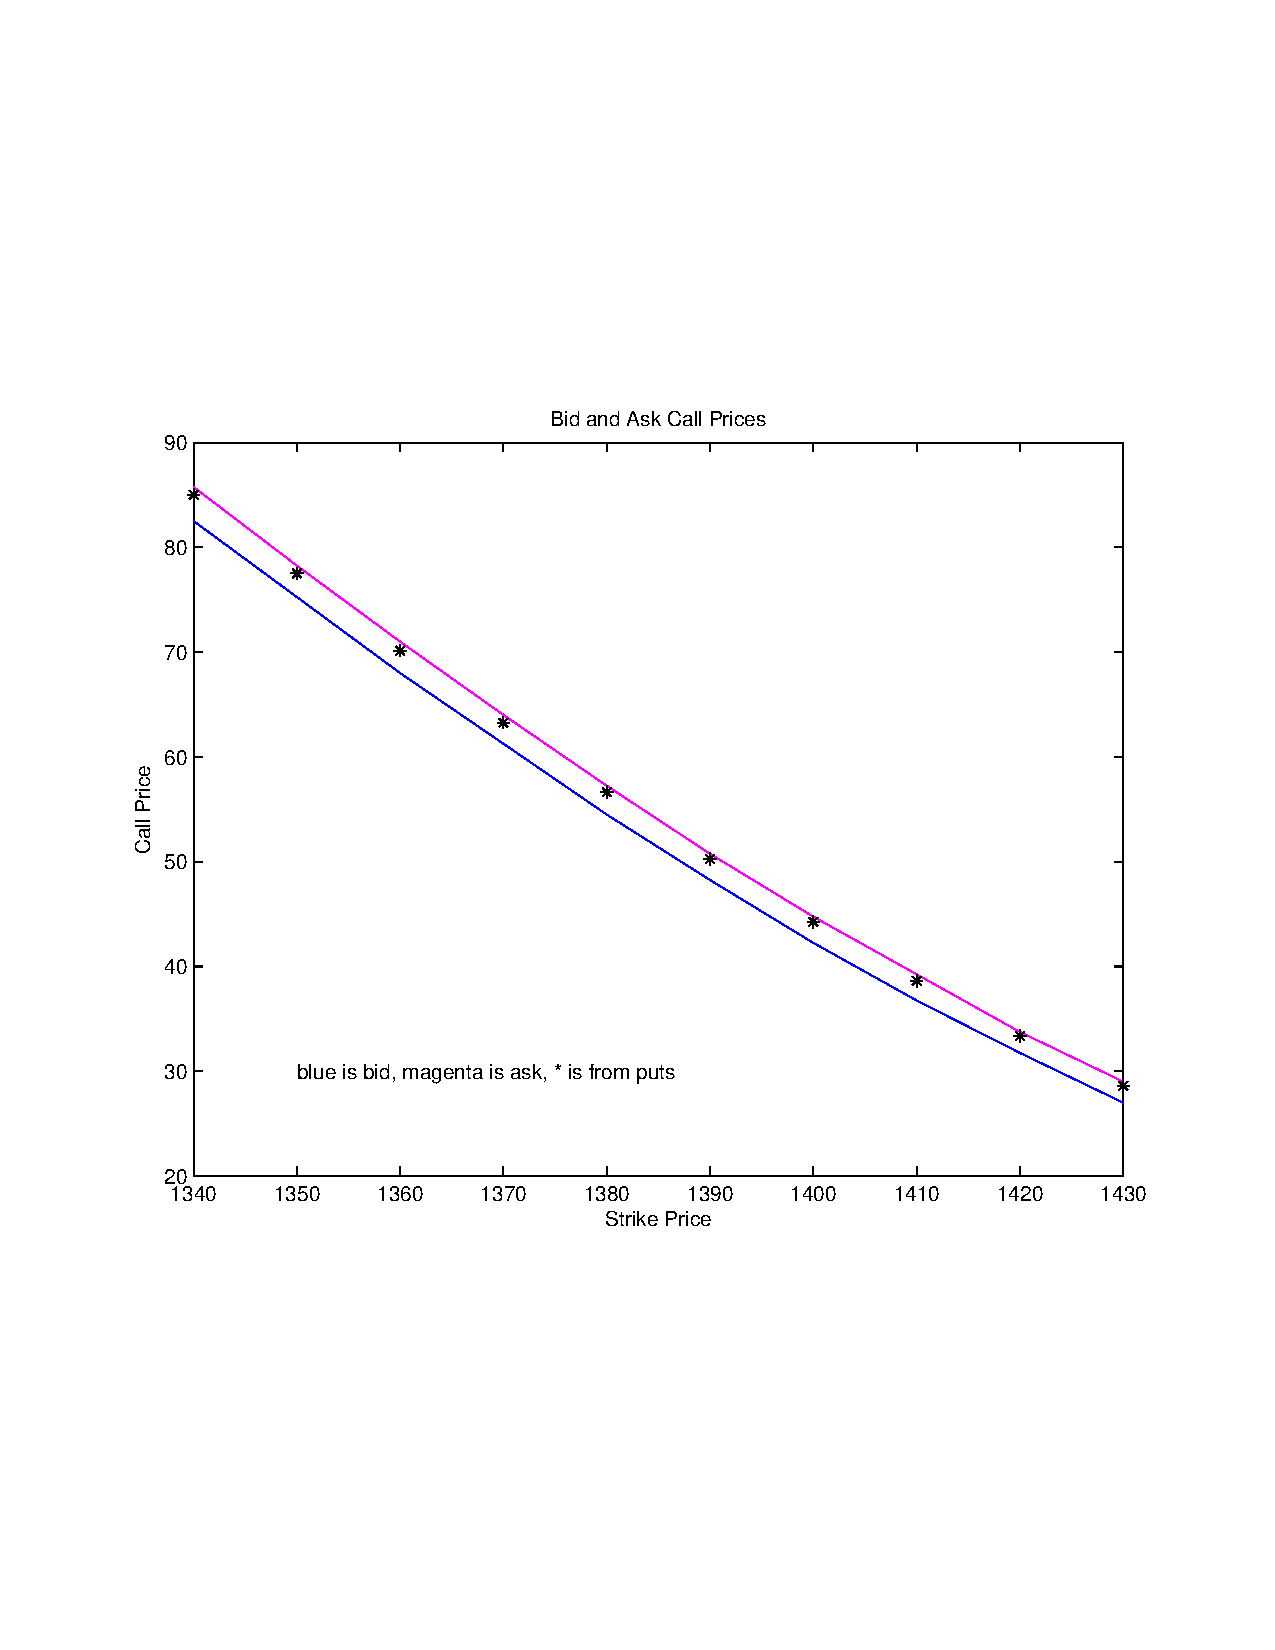
\includegraphics[width=4in]{../Matlab/hw6_q2a.pdf} \\
%%\end{center}
%%\begin{center}
%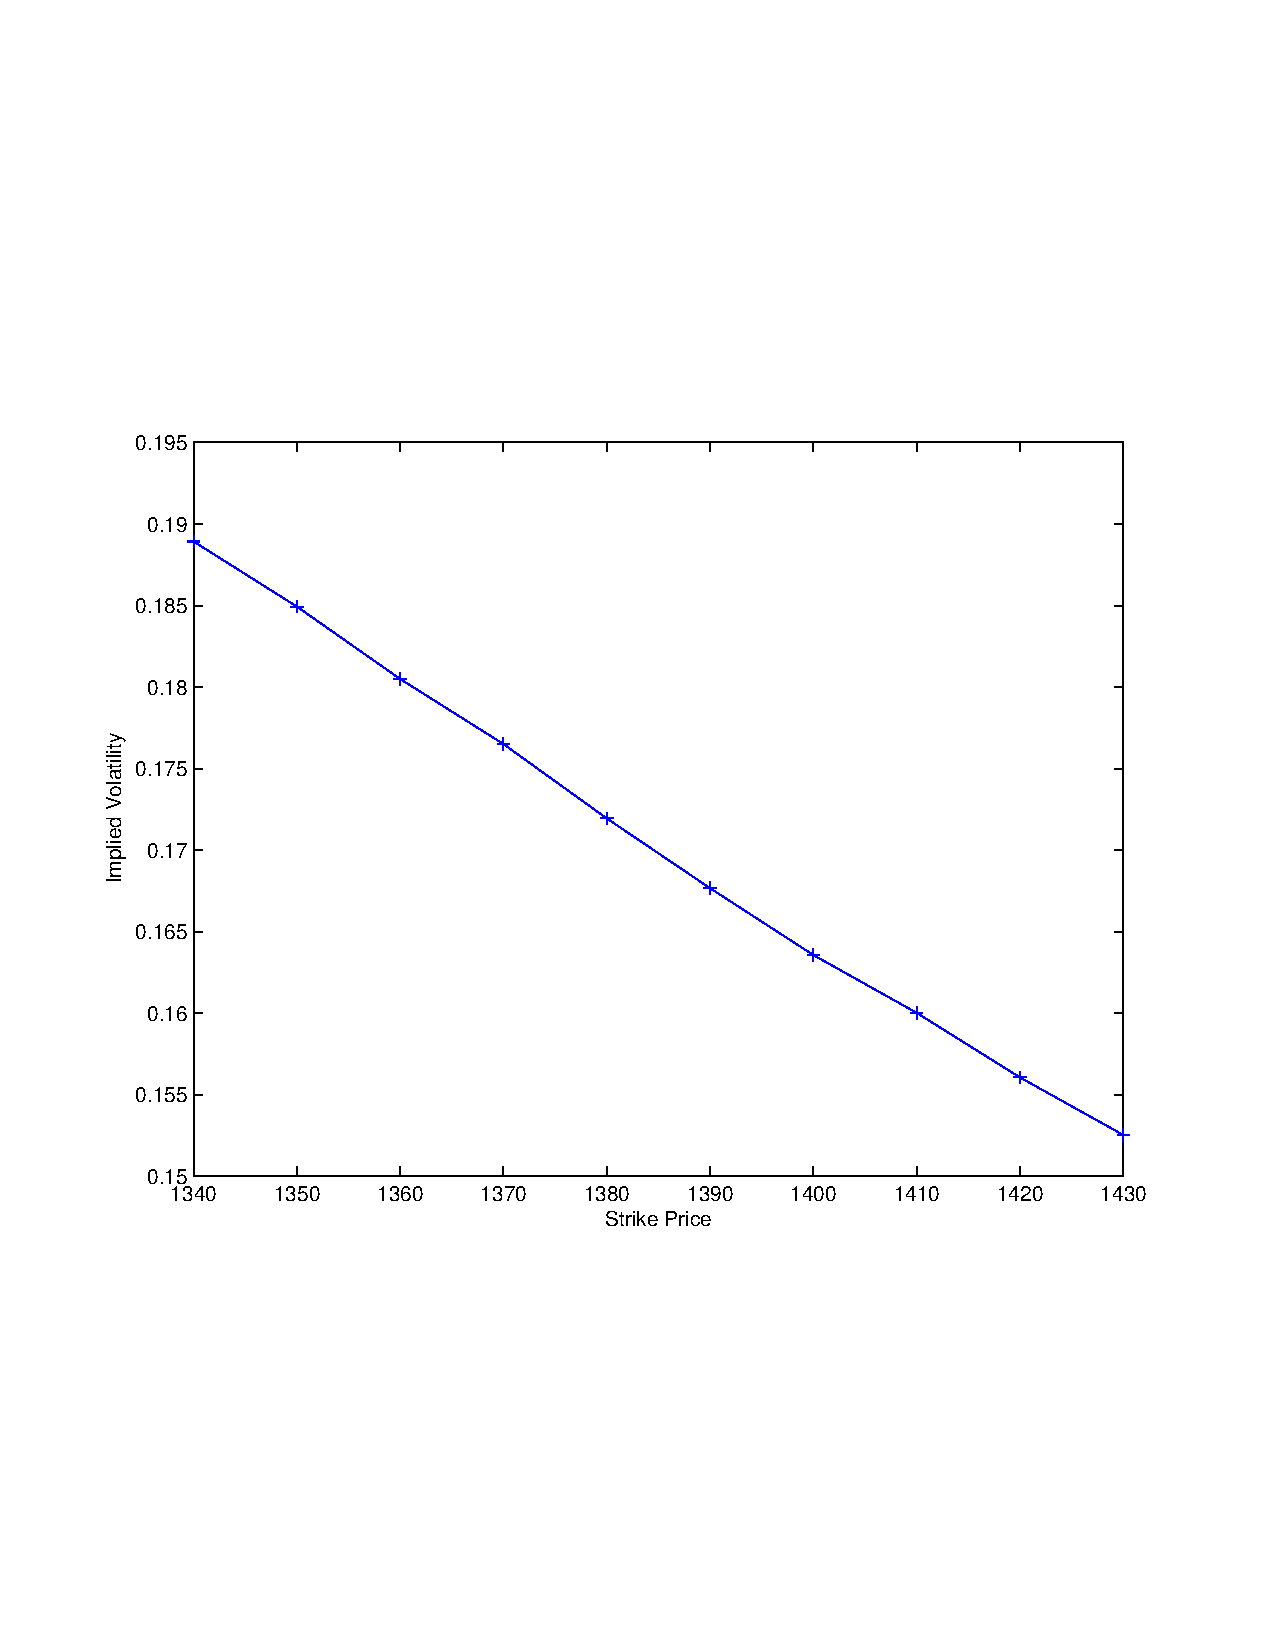
\includegraphics[width=4in]{../Matlab/hw6_q2b.pdf}
%\end{center}

\part I found option prices at \\
{\small 
\url{http://www.cmegroup.com/trading/equity-index/us-index/e-mini-sandp500.html}.
} \\
The underlying futures contract was trading at 1551.
Call options at strikes of 1550 and 1555 traded as 35.75 and 32.75.
Both are below what we saw for at-the-money options in the prices
reported above, suggesting that implied volatility is lower.
That's roughly what the VIX measures. 

\end{parts}
\end{solution}

\end{questions}

%\vfill \centerline{\it \copyright \ \number\year \ NYU Stern School of Business}

%\end{document}

%\pagebreak
{\bf Matlab program:}
\verbatiminput{../Matlab/hw6_s13.m}

%\vfill \centerline{\it \copyright \ \number\year \ NYU Stern School of Business}

\end{document}


%  EXTRA STUFF


